\chapter{Bell's Theorem}

\chapterprecis{J.~S.\ Bell} 

\makeoddhead{myheadings}{\emph{J.~S.\ Bell}}{}{\thepage}
\makeevenhead{myheadings}{\thepage}{}{\emph{Bell's Theorem}}

\renewcommand{\theequation}{\arabic{equation}}

\section*{Introduction}

The paper we are about to read takes up the issues raised by Einstein, Podolsky, and Rosen in a new way. Physicist J.~S.\ Bell gives a novel mathematical form to the suppositions of ``hidden variables'' and ``locality'' and then shows that this is in contradiction with the mathematical form of the predictions of quantum mechanics. In this chapter, we will read Bell’s original paper and then confirm by means of experiment that the particles we have been studying do not behave in the way Bell's formulation shows they would have to if they were subject to a local hidden variables theory.

The particles we have been studying are photons, but Bell makes his argument in terms of the behavior of electrons, in a special state that we have not studied. The import is the same: quantum mechanics says that two characteristics to be measured stand in a relation of mutual indeterminacy; Bell considers a situation in which two particles produced by the same process are measured separately and the supposedly indeterminate quantity in each is to be inferred from the result of the measurement of that same quantity in the other. Though the import is the same, to understand Bell’s paper, we have to understand something about the particular state and the characteristics he is talking about. The feature of interest is electron ``spin.''

\begin{figure}[!ht]
     \subfloat[Stern-Gerlach apparatus\label{subfig-1:dummy}]{%
       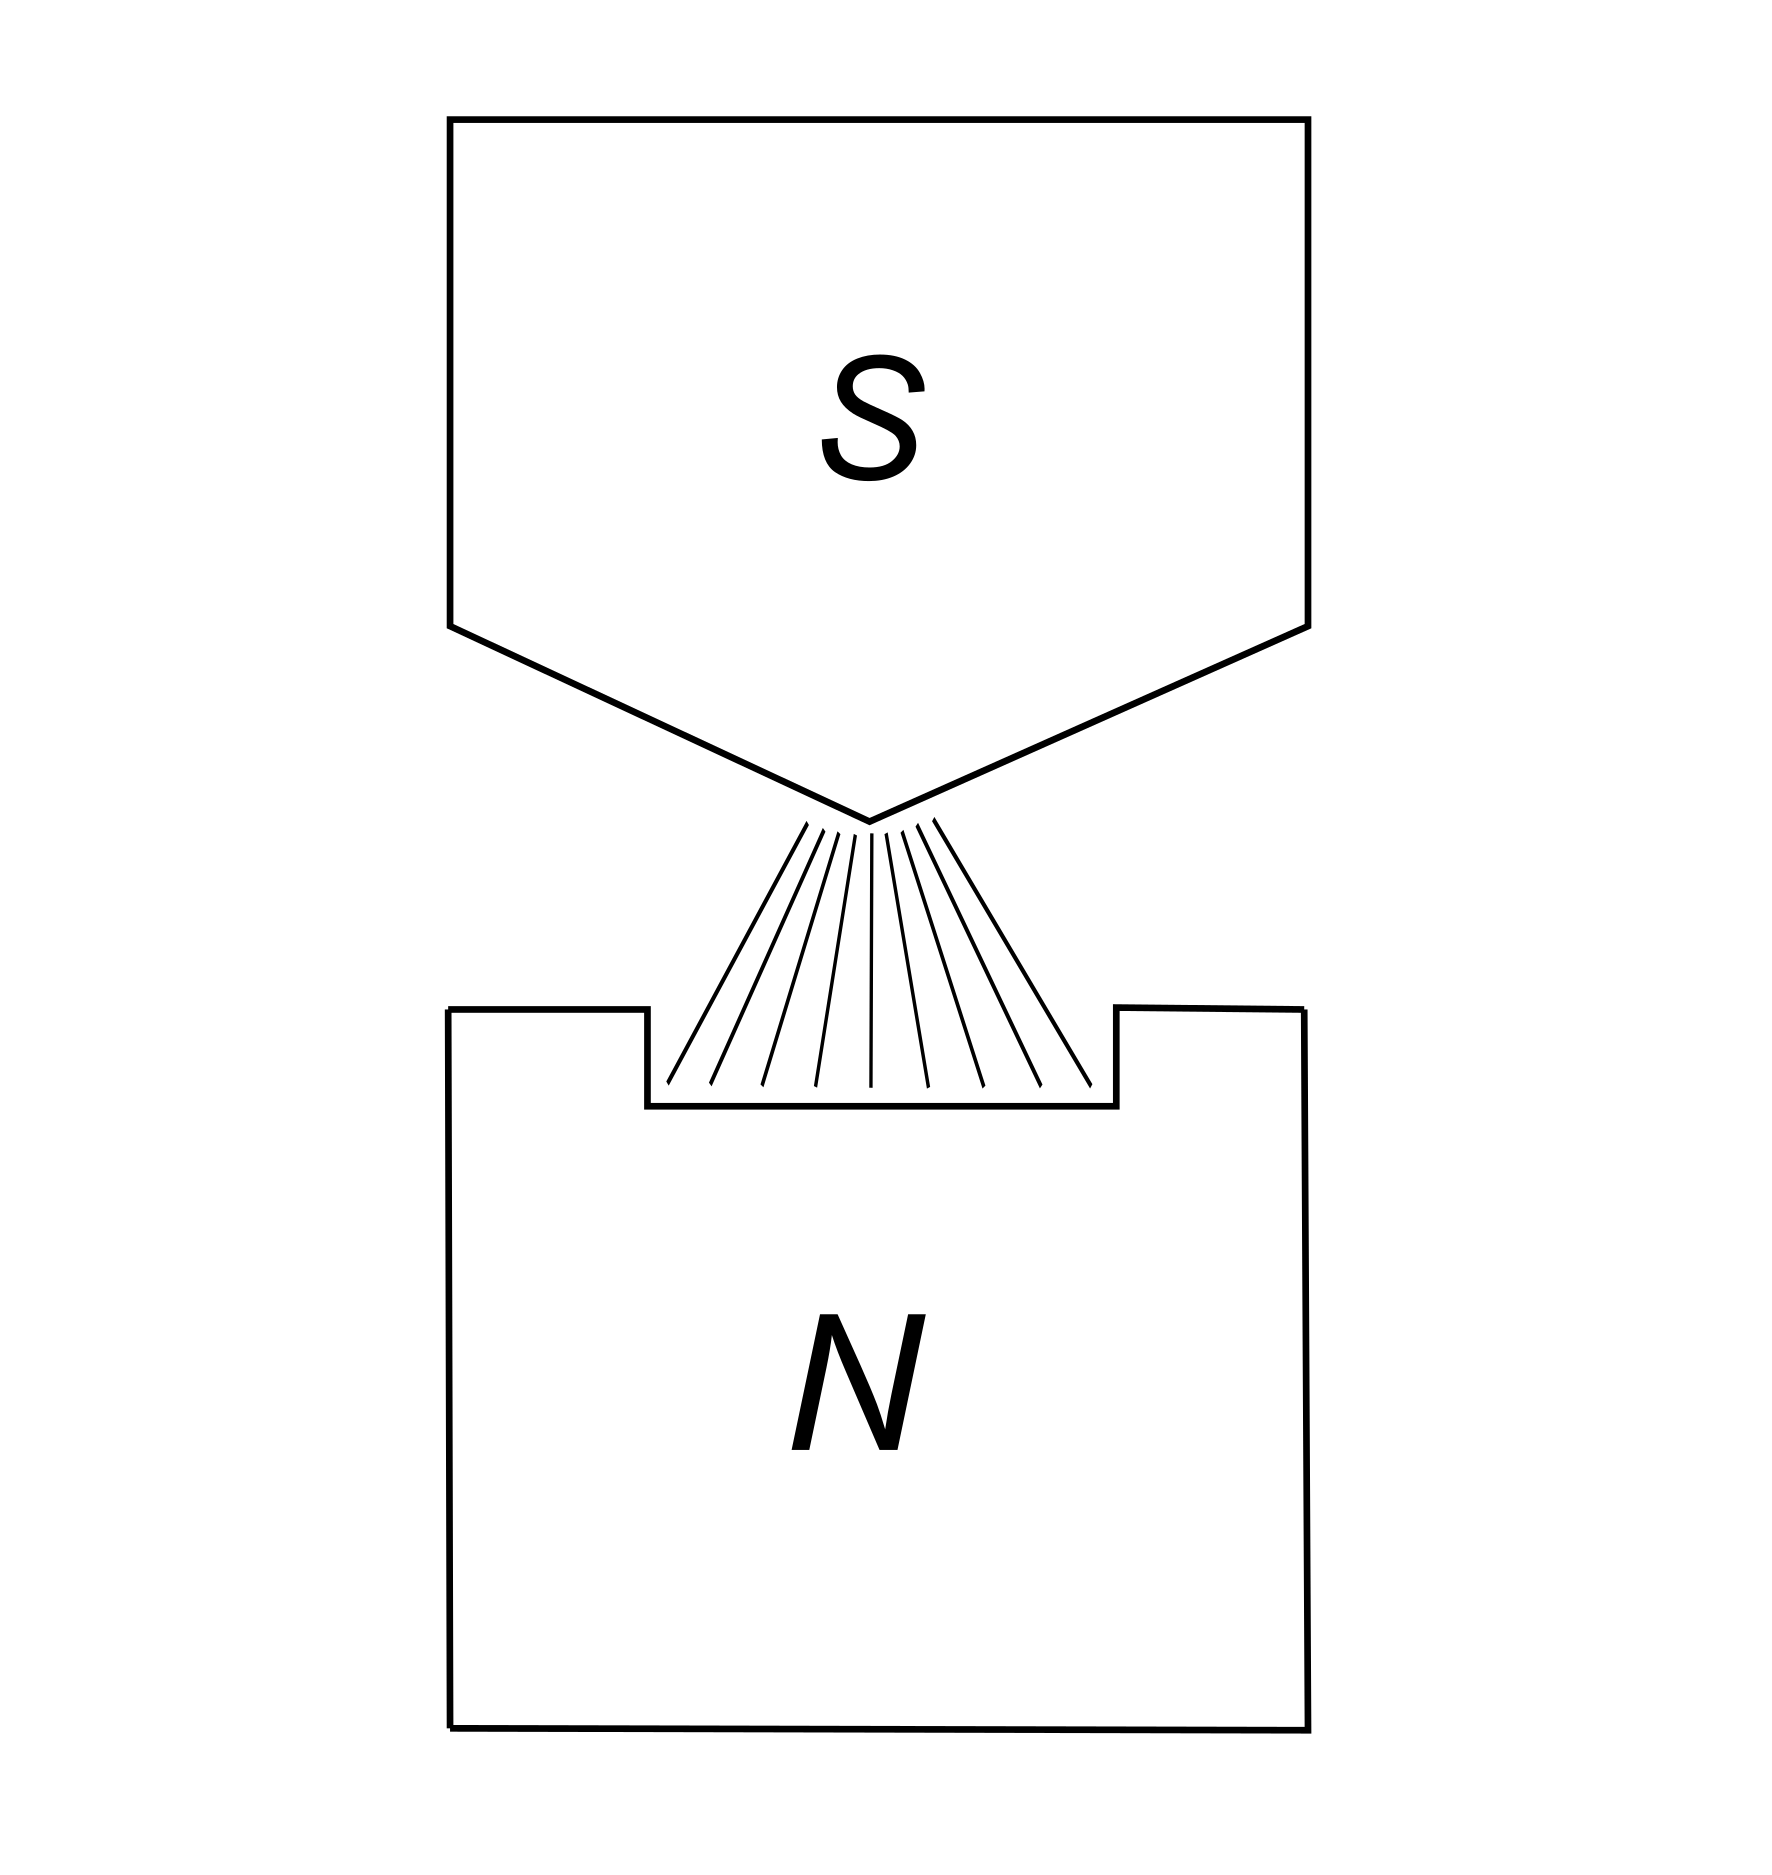
\includegraphics[width=0.45\textwidth]{images/17_bell/Stern-Gerlach.png}
     }
     \hfill
     \subfloat[Magnet in an inhomogeneous field\label{subfig-2:dummy}]{%
       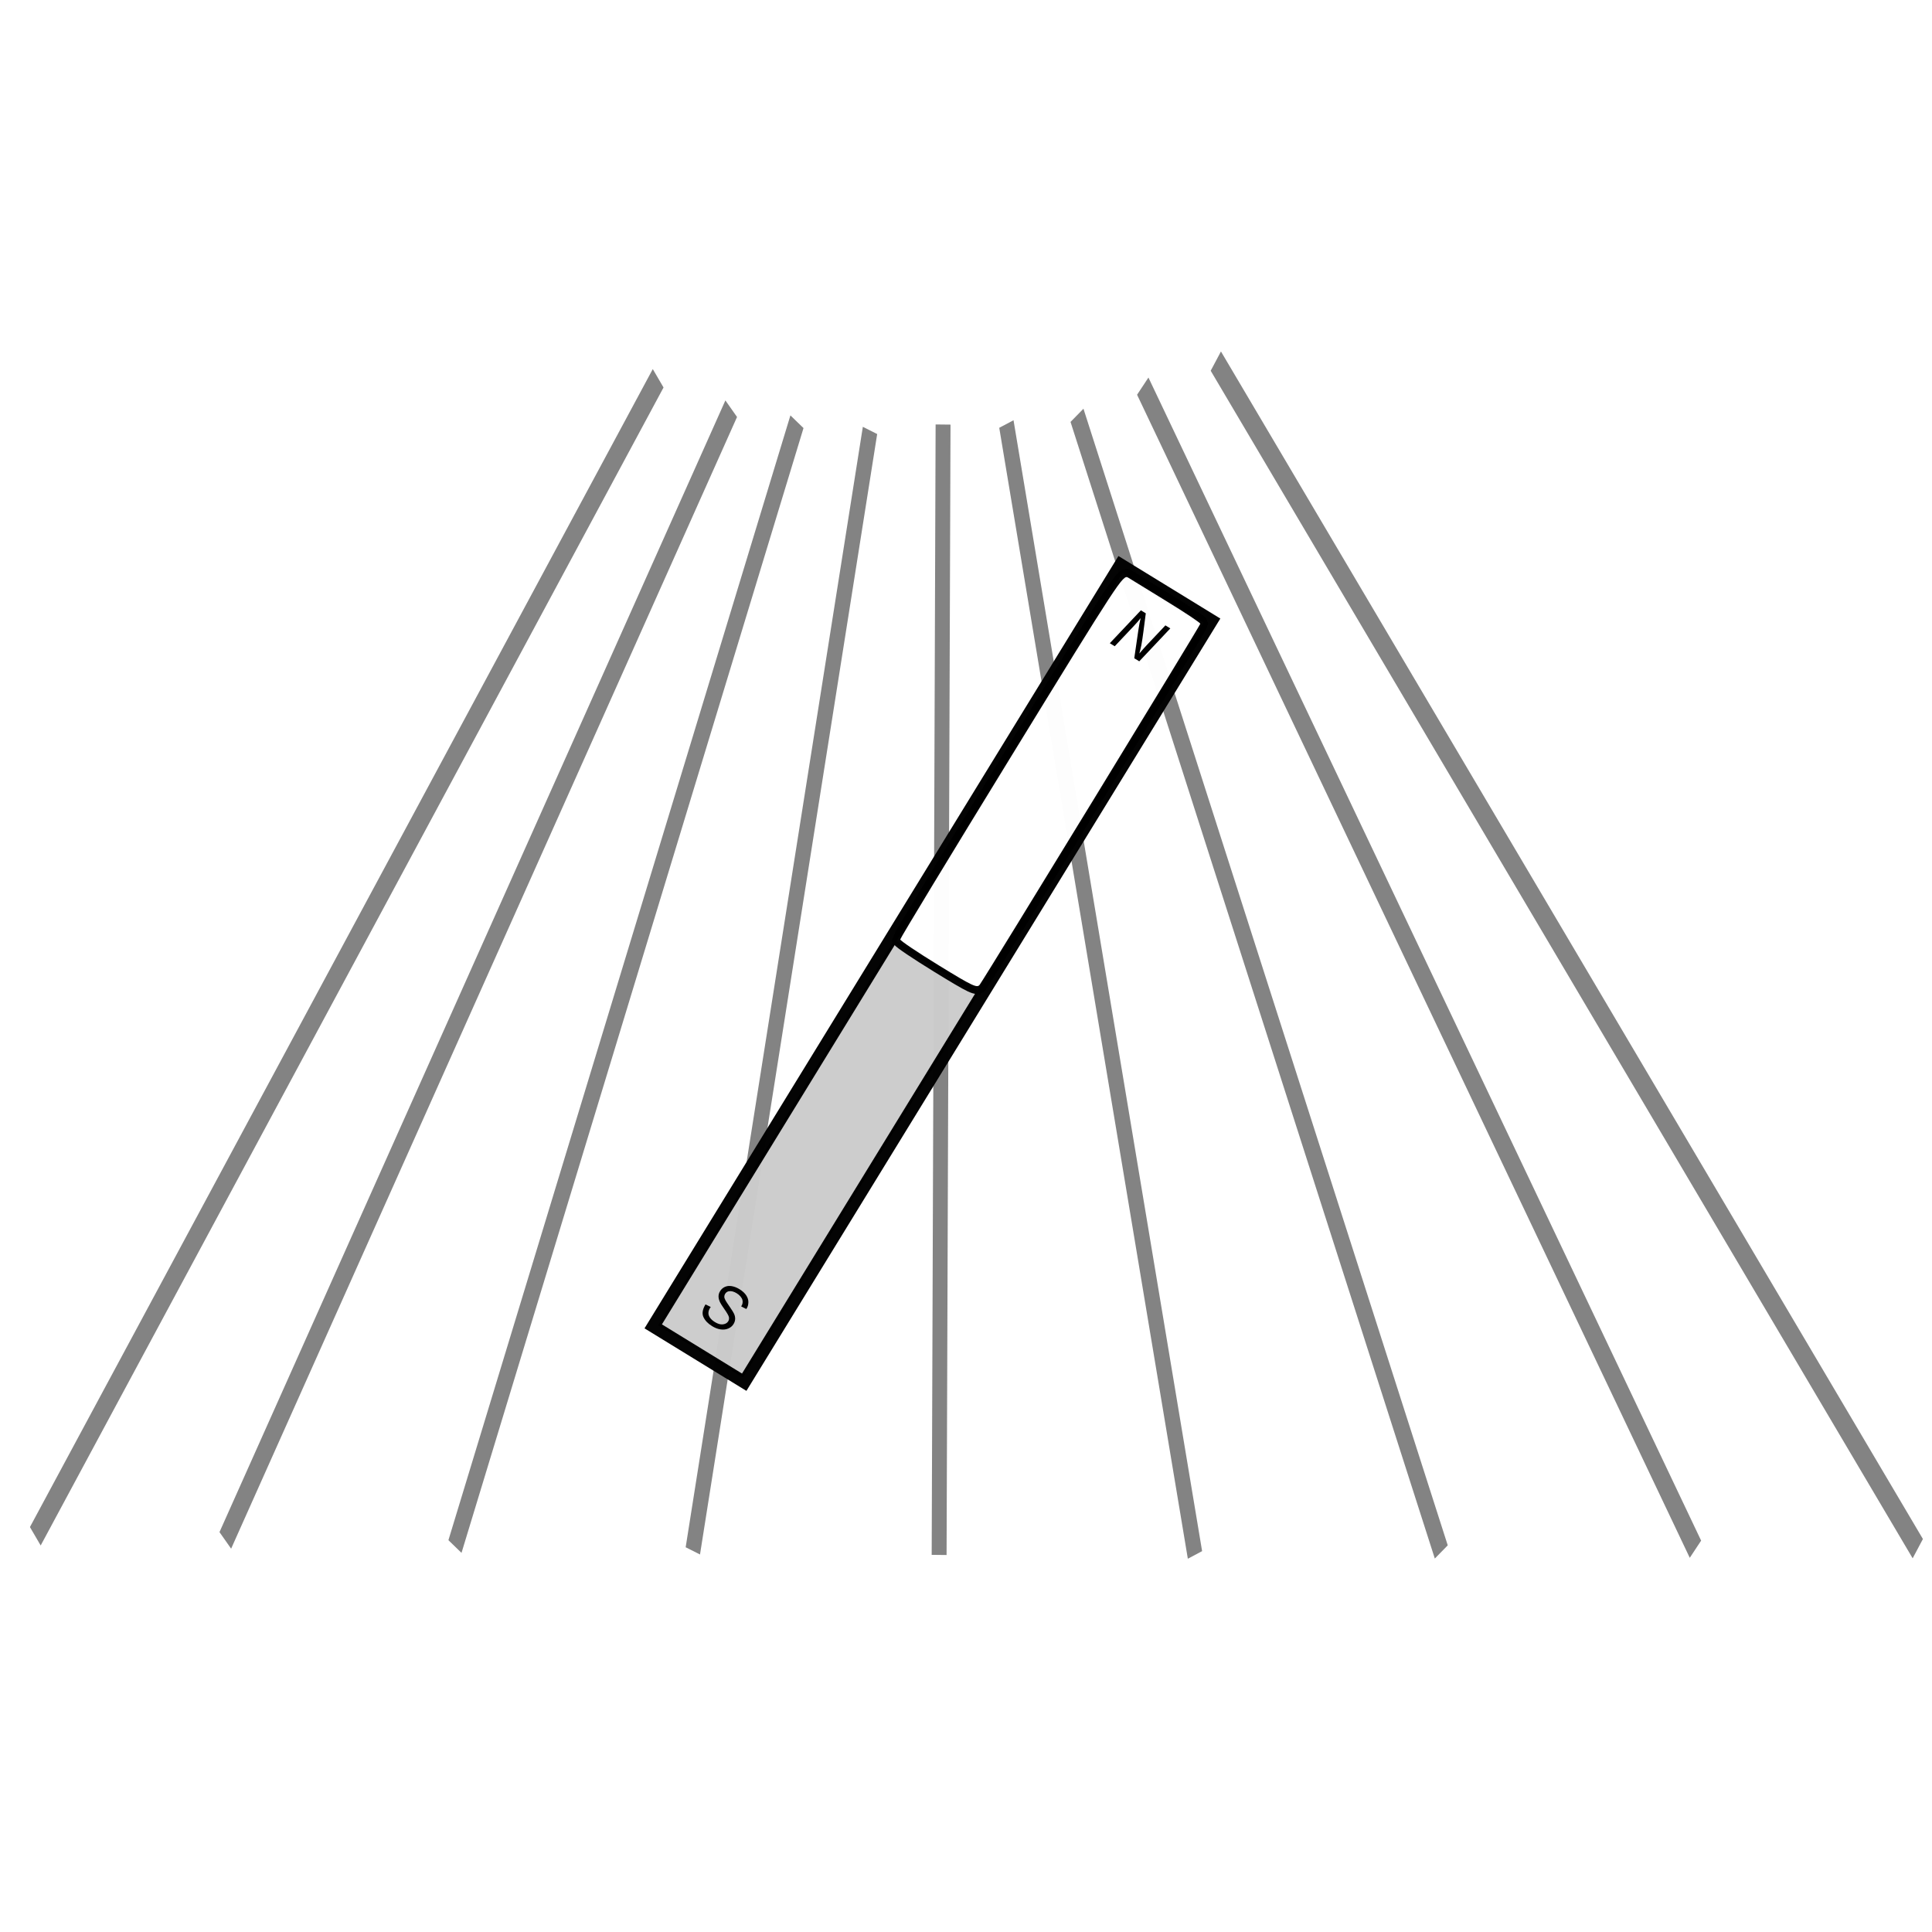
\includegraphics[width=0.45\textwidth]{images/17_bell/inhomogeneous.png}
     }
\end{figure}

In 1922, Otto Stern and Walther Gerlach performed what turned out to be a very consequential experiment, though its full significance was not recognized until years later. The experiment was conceived in order to test then-current theories of the atom based on Bohr's model. The evidence for or against the favored theory was to be found in the magnetic response of individual atoms. In particular, the revolution of the electron about the nucleus ought to count, according to Maxwell's equations, as a loop of current, effectively making the atom a tiny magnet. The theory Stern and Gerlach were testing predicted that the angular momentum of the electron measured in a particular direction ought to be quantized, just as the Bohr orbits are. The experiment consisted in firing a collimated beam of silver atoms through a powerful and inhomogeneous magnetic field like the one pictured on the left in the figure above.


Now, if the orientation of the atomic ``magnet'' were such as is pictured on the right, it would be subject not only to a counterclockwise torque, but also---since the magnetic field is stronger near the top than near the bottom (since the field lines are more concentrated there)---to a net force pulling it upwards. If many atoms were projected through the field at random orientations, some would be pulled up and some pushed down, some more and some less. If the degree of magnetization in these directions is quantized, however---that is, if the only physically meaningful answers to the question ``in which direction is this magnet oriented?'' are ``up'' and ``down''---one would expect the beam of atoms to be split, with no intermediate results. This is precisely what was found, as can be seen in the image below, taken from the original paper.

\begin{figure}[h]
  \centering
    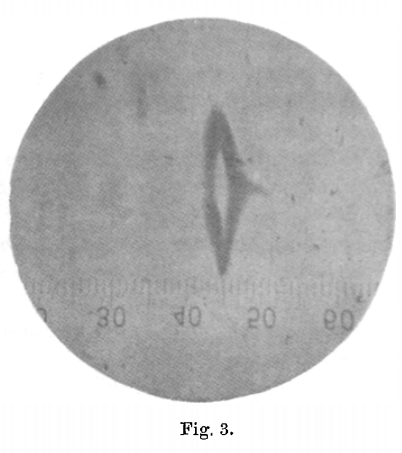
\includegraphics[width=2.00000in,height=2.00000in]{images/17_bell/result.png}
\end{figure}

Later, it was recognized that this experimental result was consistent with what the second generation of quantum-mechanical theories (\e.g., Schr\"odinger's) held, namely, that there ought to be something like an \emph{intrinsic} angular momentum, or ``spin,'' associated with the electron, one that does not result from its orbiting the nucleus, but from its inherent character. The mathematics behind this prediction are well beyond us, but the Stern-Gerlach experiment demonstrates it adequately. In our practica, we have been working with the polarization of the photon, and from the first, it has exhibited the same quantization: while a beam of light, composed of many photons, may show partial effects as described by Malus's Law, a single photon faced with a linear polarizer either passes through it or does not pass through it. Bell assumes his readers are familiar with the phenomenon of electron spin and with the apparatus for detecting it.

The quantization of intrinsic spin is of particular importance for his derivation, since he considers a pair of electrons the net spin of which is null (this is the special ``singlet spin state'' to which he refers) moving independently of one another in opposite directions, such that they can be subject to measurements at different locations. Now, quantization means that different axial directions (or ``components'') of an electron's
spin stand to one another in the ``indeterminacy relation''; that is, quantum mechanics says they cannot
in principle be assigned simultaneous reality. If the direction of an electron's spin is measured in the z-direction, quantum mechanics says it \emph{is indeterminate} in the x- and y-directions. This is the same indeterminacy relation found in Bohr's reformulation of EPR's argument, there, between the positions and momenta of two linked particles. Bell's mathematical reformulation of one version of EPR's view that quantum mechanical description of reality is importantly incomplete is notable for both its clarity and its testability. Remarks on the form of his argument follow the paper.

\section*{On The Einstein Podolsky Rosen Paradox\\
	{\large J.~S.\ Bell}}

\subsection*{I. Introduction}

The paradox of Einstein, Podolsky and Rosen\footnote{A.\ Einstein, N.\ Rosen and B.\ Podolsky, \emph{Phys.\ Rev.} \textbf{47} 777 (1935).} was advanced as an argument that quantum mechanics could not be a complete theory but should be supplemented by additional variables.  These additional variables were to restore to the theory causality and locality.\footnote{``But on one supposition we should, in my opinion, absolutely hold fast: the real factual situation of the system $S_2$ is independent of what is done with the system $S_1$, which is spatially separated from the former.'' Albert Einstein in \emph{Albert Einstein, Philosopher Scientist}, (Edited by P.\ A.\ Schilp), p.\ 85, Library of Living Philosophers, Evanston, Illinois (1949).}  In this note that idea will be formulated mathematically and shown to be incompatible with the statistical predictions of quantum mechanics.  It is the requirement of locality, or more precisely that the result of a measurement on one system be unaffected by operations on a distant system with which it has interacted in the past, that creates the essential difficulty.  There have been attempts\footnote{J.\ Von Neumann, \emph{Mathematische Grundlagen der Quanten-mechanik}, Verlag Julius-Springer, Berlin (1932), [English translation: Princeton University Press (1955)]; J.\ M.\ Jauch and C.\ Piron, \emph{Helv.\ Phys.\ Acta} \textbf{36}, 827 (1963).} to show that even without such a separability or locality requirement no ''hidden variable'' interpretation of quantum mechanics is possible.  These attempts have been examined elsewhere\footnote{J.\ S.\ Bell, to be published.} and found wanting.  Moreover, a hidden variable interpretation of elementary quantum theory\footnote{D.\ Bohm, \emph{Phys.\ Rev.}, \textbf{85}, 166 and 180 (1952).} has been explicitly constructed.  That particular interpretation has indeed a grossly non-local structure.  This is characteristic, according to the result to be probed here, of any such theory which reproduces exactly the quantum mechanical predictions.

\subsection*{II. Formulation}

With the example advocated by Bohm and Aharonov,\footnote{D.\ Bohm and Y.\ Aharonov, \emph{Phys.\ Rev.} \textbf{108}, 1070 (1957).} the EPR argument is the following. Consider
a pair of spin one-half particles formed somehow in the singlet spin state and moving freely in opposite
directions. Measurements can be made, say by Stern-Gerlach magnets, on selected components of the
spins $\pmb{\sigma}_1$ and $\pmb{\sigma}_2$. If measurement of the component $\pmb{\sigma}_1 \cdot \pmb{a}$, where $\pmb{a}$ is some unit vector, yields the value $+1$ then, according to quantum mechanics, measurement of $\pmb{\sigma}_2 \cdot \pmb{a}$ must yield the value $-1$ and vice versa.\footnote{[In some physical processes akin to those envisaged by EPR (e.g., the ``singlet spin state''), one component of the direction of spin $\pmb{\sigma}_2$ (the component in the direction $\pmb{a}$) could be inferred, without disturbing it, from the result of a measurement of that same component in the spin $\pmb{\sigma}_1$ of its counterpart. Symbolically, this latter measurement is expressed as the ``dot product'' of the two vectors: $\pmb{\sigma}_1 \cdot \pmb{a}$. Briefly, if two unit vectors span an angle $\theta$, their dot product yields $\cos \theta$, ranging from $+1$ when the vectors point in the same direction, through $0$ when they are perpendicular, to $-1$ when they point in opposite directions. As we saw from the Stern-Gerlach experiment, though, electron spin is quantized, so there are only two possible outcomes of the measurements: the spin of the particle points in the direction measured ($+1$) or it points in the opposite direction ($-1$). The use of the dot product here, then, is somewhat loose, connoting a general comparison of directions.]}
Now we make the hypothesis [of Einstein, cited above], and it seems one at least worth considering, that if the two measurements
are made at places remote from one another the orientation of one magnet does not influence the
result obtained with the other. Since we can predict in advance the result of measuring any chosen component
of $\pmb{\sigma}_2$, by previously measuring the same component of $\pmb{\sigma}_1$, it follows that the result of any such
measurement must actually be predetermined. Since the initial quantum mechanical wave function does not
determine the result of an individual measurement, this predetermination implies the possibility of a more
complete specification of the state.

Let this more complete specification be effected by means of parameters $\lambda$. It is a matter of indifference
in the following whether $\lambda$ denotes a single variable or a set, or even a set of functions, and whether
the variables are discrete or continuous. However, we write as if $\lambda$ were a single continuous parameter.
The result $A$ of measuring $\pmb{\sigma}_1 \cdot \pmb{a}$ is then determined by $\pmb{a}$ and $\lambda$, and the result $B$ of measuring 
$\pmb{\sigma}_2 \cdot \pmb{b}$ in the same instance is determined by $\pmb{b}$ and $\lambda$, and
%
\begin{equation}\label{eq:bell_1} % eqn 1
A(\pmb{a}, \lambda) = \pm1; B(\pmb{b}, \lambda) = \pm 1.
\end{equation}
%
The vital assumption [of the quote from Einstein] is that the result $B$ for particle $2$ does not depend on the setting $\pmb{a}$ of the magnet
for particle $1$, nor $A$ on $\pmb{b}$.\footnote{[Bell is here highlighting what is significant about the functional notation in equation \eqref{eq:bell_1}, namely, that the results of the measurements $A$ and $B$ are determined completely and solely by the variables listed in their definitions.]} 

If $\rho(\lambda)$ is the probability distribution of $\lambda$ then the expectation value of the product of the two 
components $\pmb{\sigma}_1 \cdot \pmb{a}$ and $\pmb{\sigma}_2 \cdot \pmb{b}$ is\footnote{[According to the hypothesis Bell is investigating, the ``more complete specification'' of the particles' state, the extra information that would tell the observer who knew it which way the particle would respond to a given measurement, is given by $\lambda$. Equation \eqref{eq:bell_2} considers all the possible $\lambda$'s and weights them according to how likely each is. Mathematically, that means integrating over all the possible values of $\lambda$ and weighting each by its likelihood, represented by the probability distribution $\rho(\lambda)$. It may be helpful to note that $P$ was likely chosen to stand for ``product,'' since the term we are integrating $\rho$ against is the product of $A$ and $B$. Because we have defined $A$ and $B$ such that the results of measurements yield the values $+1$ and $-1$, the product for any given value of $\lambda$ will always be either $+1$ (meaning that the two particles would both be measured to be pointing either in the selected directions $\pmb{a}$ and $\pmb{b}$ or in directions opposed to them) or $-1$ (meaning that the directions of $\pmb{\sigma}_1$ and $\pmb{\sigma}_2$ would be measured to be opposed, whether because $\pmb{\sigma}_1$ would \emph{not} be measured to point in direction $\pmb{a}$ and $\pmb{\sigma}_2$ \emph{would} be measured to point in direction $\pmb{b}$ or because $\pmb{\sigma}_1$ \emph{would} be measured to point in direction $\pmb{a}$ and $\pmb{\sigma}_2$ would \emph{not} be measured to point in direction $\pmb{b}$). Since it is a weighted sum of all the positive and negative terms, $P(\pmb{a},\pmb{b})$ is thus a measure of the \emph{correlation} between the spin-direction of the two particles relative to the angles $\pmb{a}$ and $\pmb{b}$.]}
\begin{equation}\label{eq:bell_2} % eqn 2
P(\pmb{a}, \pmb{b}) = \int d\lambda\, \rho(\lambda) A(\pmb{a}, \lambda) B(\pmb{b}, \lambda).
\end{equation}
This should equal the quantum mechanical expectation value, which for the singlet state is\footnote{[As for the left-hand side, the angle brackets denote an average, that of the product of the results of the measurements described in the previous note, taken for many pairs of electrons. As for the right-hand side, since $\pmb{a}$ and $\pmb{b}$ are unit vectors, their dot product can take on any value from $-1$, when they are pointing in opposite directions, to $+1$, when they are pointing in the same direction. Again, for any two unit-length vectors spanning an angle $\theta$, their dot product is equal to $\cos \theta$. The minus sign denotes the theoretical expectation that the spins will be opposed. So, if $\pmb{a}$ and $\pmb{b}$ point in the same direction, the result will be $-\cos 0^{\circ} = -1$. A key move for the experiment will be to take measurements in directions that are neither opposed nor identical, since they will involve components the theory says are in the indeterminacy relation. In this usage, then, the dot product is meant perfectly literally.]}
\begin{equation}\label{eq:bell_3} %eqn 3
< \pmb{\sigma}_1 \cdot \pmb{a} \  \pmb{\sigma}_2 \cdot \pmb{b} >\  = - \pmb{a} \cdot \pmb{b} .
\end{equation}
%
But it will be shown that this is not possible.

Some might prefer a formulation in which the hidden variables fall into two sets, with $A$ dependent on
one and $B$ on the other; this possibility is contained in the above, since $\lambda$ stands for any number of variables
and the dependences thereon of $A$ and $B$ are unrestricted. In a complete physical theory of the
type envisaged by Einstein, the hidden variables would have dynamical significance and laws of motion;
our $\lambda$ can then be thought of as initial values of these variables at some suitable instant.\\
\centerline{* * *}
%
\subsection*{IV. Contradiction}

The main result will now be proved. Because $\rho$ is a normalized probability distribution,

\setcounter{equation}{11}

\begin{equation}
\int d\lambda\, \rho(\lambda) = 1,
\end{equation}
and because of the properties \eqref{eq:bell_1}, $P$ in \eqref{eq:bell_2} cannot be less than $-1$. It can reach $-1$ at $\pmb{a} = \pmb{b}$ only if
\begin{equation}
A(\pmb{a}, \lambda) = - B(\pmb{a}, \lambda)
\end{equation}
except at a set of points $\lambda$ of zero probability. Assuming this, \eqref{eq:bell_2} can be rewritten
\begin{equation}
P(\pmb{a}, \pmb{b}) = - \int d\lambda\, \rho(\lambda) A(\pmb{a}, \lambda) A(\pmb{b}, \lambda).
\end{equation}

It follows that if $\pmb{c}$ is another unit vector
\begin{align*}
P(\pmb{a}, \pmb{b}) - P(\pmb{a}, \pmb{c}) &= - \int d\lambda\, \rho(\lambda) [A(\pmb{a}, \lambda) A(\pmb{b}, \lambda) - A(\pmb{a}, \lambda) A(\pmb{c}, \lambda)] \\
 &= \int d\lambda\, \rho(\lambda) A(\pmb{a}, \lambda) A(\pmb{b}, \lambda) [A(\pmb{b}, \lambda) A(\pmb{c}, \lambda)-1],
\end{align*}
using \eqref{eq:bell_1},\footnote{[Since $A(\pmb{b},\lambda)A(\pmb{b},\lambda)=1$ for any $\pmb{b}$ and any $\lambda$.]} whence\footnote{[The introduction of the inequality depends on two points. The definition of $A$ in \eqref{eq:bell_1} implies that the average value of $A(\pmb{a}, \lambda) A(\pmb{b}, \lambda)$ can range from $-1$ to $+1$; furthermore, $\rho(\lambda)[1 - A(\pmb{b}, \lambda) A(\pmb{c}, \lambda)] \geq 0$. This and the previous footnote are based on David J.\ Griffiths (\emph{Introduction to Quantum Mechanics}, Upper Saddle River, NJ: Pearson Prentice Hall, 2005), 437.]}
\begin{equation*}
|P(\pmb{a}, \pmb{b}) - P(\pmb{a}, \pmb{c})| \leq \int d\lambda\, \rho(\lambda) [1 - A(\pmb{b}, \lambda) A(\pmb{c}, \lambda)].
\end{equation*}
The second term on the right is $P(\pmb{b}, \pmb{c})$, whence
\begin{equation}
1 + P(\pmb{b}, \pmb{c}) \geq |P(\pmb{a}, \pmb{b}) - P(\pmb{a}, \pmb{c})|.
\end{equation}
Unless $P$ is constant, the right hand side is in general of order $|\pmb{b}-\pmb{c}|$ for small $|\pmb{b}-\pmb{c}|$. Thus $P(\pmb{b}, \pmb{c})$
cannot be stationary at the minimum value ($-1$ at $\pmb{b} = \pmb{c}$) and cannot 
equal the quantum mechanical value \eqref{eq:bell_3}.\footnote{[See the Remarks after the paper for discussion of this and the previous sentence.]}\\
\centerline{* * *}

\subsection*{V. Generalization}
The example considered above has the advantage that it requires little imagination to envisage the
measurements involved actually being made\ldots. [F]or at least one quantum state, the ``singlet'' state \ldots\,the 
statistical predictions of quantum mechanics are incompatible with separable predetermination.

\subsection*{VI. Conclusion}
In a theory in which parameters are added to quantum mechanics to determine the results of individual
measurements, without changing the statistical predictions, there must be a mechanism whereby the setting
of one measuring device can influence the reading of another instrument, however remote. Moreover,
the signal involved must propagate instantaneously, so that such a theory could not be Lorentz invariant.
Of course, the situation is different if the quantum mechanical predictions are of limited validity.
Conceivably they might apply only to experiments in which the settings of the instruments are made sufficiently
in advance to allow them to reach some mutual rapport by exchange of signals with velocity less
than or equal to that of light. In that connection, experiments of the type proposed by Bohm and Aharonov, in which the settings are changed during the flight of the particles, are crucial.

\section*{Remarks}

Bell's "note" demonstrates a contradiction, and like any \emph{reductio ad absurdum,} therefore, 
demonstrates that an inconsistency lurks somewhere in the premises it is testing. He seems to
identify one as the source of the problem when he writes: 
\begin{quote}
It is the \emph{requirement of locality,} or more precisely that the result of a measurement on one system be unaffected by operations on a distant system with which it has interacted in the past, that creates the essential difficulty.
\end{quote}
However that may be, the import of his argument has been interpreted variously, with many identifying the idea of complete determinacy or ``hidden'' variables as the essential problem. A main goal of these remarks is to clarify its logical structure. Afterwards, we will confirm by means of experiment the "statistical predictions of quantum mechanics" that are in contradiction with the sort of "local hidden variables theory" that is developed in the course of Bell's argument, though in a form different from the one he envisages, using photon polarization instead of electron spin.

As for the argument, in section II, Bell reformulates EPR's proposal in the experimentally suggestive terms formulated by Bohm and Aharonov. The essential feature is the same, namely, two
particles with a known relation (in this case, that their spins are opposed) are produced 
by a process predicted by quantum mechanics, one that happens to send the particles away from 
each other, such that their individual states might be measured separately. Just as in the case
of ordinary polarization that Dirac discusses, the description that quantum mechanics gives of these particles involves a superposition of states, leading to a merely probabilistic prediction of the outcome. In the case of particles that stand in the uncertainty relation,\footnote{A mathematically precise way of specifying which physical quantities stand in that relation is developed in later chapters of Dirac's \emph{Principles of Quantum Mechanics,} and it is this formalism, that of ``non-commuting observables'' that EPR refer to in their 1935 paper.} EPR show that the quantum-mechanical description does not contain enough information to tell how either will react; as they conclude, "the wave function does not provide a complete description of the physical reality."

This is where Bell's reformulation comes in, with the definitions of the measurement results $A$ and
$B$ and the expectation value of their product $P$ in equations (1) and (2), all in terms of the "more complete specification of the state" embodied in the term $\lambda$. The predictions of quantum
mechanics are embodied in equation (3), which here plays a role analogous to that of Bohr's 
considerations (see note \ref{entangle} in Chapter \ref{EPR}, page \pageref{entangle}), concerning the momentum relation between the spatially 
separated systems (the relation that allows a measurement on one to reveal something about the state
of the other). A hybridization of the two accounts could be said to occur in equation (13), 
the special case where the orientations of the detectors ($\pmb{a} \text{ and } \pmb{b}$) are the same,
such that the dot product in equation (3) yields the value $-1$. Bell exploits this case to set a
further specification on the functions $A$ and $B$: whatever else they may say, they must
be such that for the \emph{same} angle, they predict numerically opposed results. $A(\pmb{a},\lambda)$
must equal the negative of $B(\pmb{a},\lambda)$. As a result, equation (14) recasts equation (2)---the equation that indicates how to calculate the correlation of the two measurements---in a form that combines the statistical predictions of quantum mechanics with the idea that the measurements are independent and determined in
advance by $\lambda$. At this point, the deed is done: locality and determinacy have been represented mathematically. The introduction of a third angle and a few simple substitutions and rearrangements will yield Bell's inequality, equation (15), which, we will demonstrate, stands in contradiction with the experimentally verified predictions of equation (3).

So much for an account of the arc of the argument. The all-too-brief sentences following equation (15), detailing the contradiction, require 
significant elucidation, which will take up the remainder of this subsection. At this point, Bell might simply have chosen some values for the angles $\pmb{a}, \pmb{b},$  and $\pmb{c}$ that would make the values
equation (3) predicts for the expectation values $P(\pmb{a}, \pmb{b}), P(\pmb{a}, \pmb{c}),$ and
$P(\pmb{b}, \pmb{c})$ violate the inequality. Arguably, there is something more
satisfying in demonstrating a more general result: showing that for a whole \emph{range} of possible 
values, the inequality is violated. 
He accomplishes this by pointing out that when
$\pmb{b}$ and $\pmb{c}$ are close (or in his words, "for small $|\pmb{b} - \pmb{c}|$"),
the left-hand side of (15) is expected according to equation (3) to be "stationary" at the value 0.
(What he actually talks about is $P(\pmb{b}, \pmb{c})$ being stationary at $-1$, but since this
is added to the constant 1, it amounts to the same.) If the left-hand side is stationary at a minimum
of 0 when $\pmb{b}$ and $\pmb{c}$ are close, this means qualitatively that its graph in that region is "flat."
By contrast, Bell points out, the right-hand side "is \ldots of order $|\pmb{b} - \pmb{c}|$," the
absolute value of the difference between the two angles; the graph of this, too, reaches a minimum
of 0 when the angles are equal, but instead of being flat, is "pointy." In the region around 0, the graph that is 
pointy inevitably lies \emph{above} the graph that is flat, but the right-hand side is meant to be less
than or equal to the left, if the inequality holds. Thus, Bell's words in section IV about $P(\pmb{b}, \pmb{c})$---that it "cannot be stationary" and "cannot equal the quantum mechanical value"---have the silent proviso 
"while equation (15) holds and $P(\pmb{a},\pmb{b})$ and $P(\pmb{a},\pmb{c})$ have their 
quantum-mechanical values."

A quantitative derivation of this contradiction follows. For the left-hand side of (15), 
since $P(\pmb{b}, \pmb{c})$ by (3) ought to equal $-\pmb{b} \cdot \pmb{c}$, we can put $1 - \cos (\pmb{b}-\pmb{c})$.
The right-hand side is trickier, and will require a few approximations and interpolations. First, we
will apply equation (3) to get the expected value of the products: $P(\pmb{a},\pmb{b}) = - \cos (\pmb{a}-\pmb{b})$
and $P(\pmb{a},\pmb{c}) = - \cos(\pmb{a}-\pmb{c})$. Accordingly, we rewrite the right-hand side of (15) as
\begin{equation*}\tag{15a -- RHS}
|P(\pmb{a},\pmb{b})-P(\pmb{a},\pmb{c})| = |- \cos(\pmb{a}-\pmb{b}) + \cos(\pmb{a}-\pmb{c})|.
\end{equation*}
Now, the argument of the rightmost term ($\pmb{a}-\pmb{c}$) can be rewritten as $(\pmb{a}-\pmb{b}) + (\pmb{b}-\pmb{c})$.
According to the rule for the cosine of a sum of angles, $\cos(F + G) = \cos F \cos G - \sin F \sin G$. Hence,
\begin{equation*}
\cos [(\pmb{a}-\pmb{b}) + (\pmb{b}-\pmb{c})] 
= \cos(\pmb{a}-\pmb{b}) \cos(\pmb{b}-\pmb{c}) - \sin(\pmb{a}-\pmb{b}) \sin(\pmb{b}-\pmb{c}).
\end{equation*}
You may already be familiar with the small-angle approximation for the sine function, $\sin x \approx x$, used
in Junior Lab in discussing the motion of the pendulum. There is an analogous approximation for cosine, 
$\cos x \approx 1 - \frac{x^2}{2}$. Therefore, using both for the terms involving $(\pmb{b}-\pmb{c})$,
\begin{equation*}
\cos(\pmb{a}-\pmb{b}) \cos(\pmb{b}-\pmb{c}) - \sin(\pmb{a}-\pmb{b}) \sin(\pmb{b}-\pmb{c})
= \cos(\pmb{a}-\pmb{b}) [1-(\pmb{b}-\pmb{c})^2/2] - \sin(\pmb{a}-\pmb{b}) (\pmb{b}-\pmb{c}).
\end{equation*}
Substituting this back into our (15a -- RHS) above, we get
\begin{equation*}\tag{15b -- RHS}
|- \cos(\pmb{a}-\pmb{b}) + \cos(\pmb{a}-\pmb{b}) - \cos(\pmb{a}-\pmb{b})(\pmb{b}-\pmb{c})^2/2 -
\sin(\pmb{a}-\pmb{b}) (\pmb{b}-\pmb{c})|.
\end{equation*}

Now, since $\pmb{a}$ and $\pmb{b}$ are just some constant angles, the
terms $\cos(\pmb{a}-\pmb{b})/2$ and $\sin(\pmb{a}-\pmb{b})$, also, are just some constants $X$ and 
$Y$ ranging from $-$\textonehalf\  to $+$\textonehalf\  and from $-1$ to $+1$ respectively. It follows that 
we can rewrite the right-hand side of (15) as a function of $\pmb{b}-\pmb{c}$,
\begin{equation*}\tag{15c -- RHS}
|P(\pmb{a},\pmb{b})-P(\pmb{a},\pmb{c})| = |X(\pmb{b}-\pmb{c})^2 + Y(\pmb{b}-\pmb{c})|.
\end{equation*}
This contains one term that is linear in $\pmb{b}-\pmb{c}$ and one that is quadratic in 
$\pmb{b}-\pmb{c}$.
For small values of $|\pmb{b}-\pmb{c}|$, much less than 1, the linear term ($Y(\pmb{b}-\pmb{c})$) will dominate 
and the quadratic term (much, much smaller) can effectively be disregarded. This is what justifies
Bell in his assertion that ``the right hand side is in general of order $|\pmb{b}-\pmb{c}|$ for 
small $|\pmb{b}-\pmb{c}|$.''

For illustration, we take the case in which $\pmb{a}-\pmb{b}$ is equal to 45$^\circ$, and graph
the left and right hand sides of Bell's equation (15) for values of $\pmb{b}-\pmb{c}$ near 0.

\begin{figure}[h]
  \begin{center}
    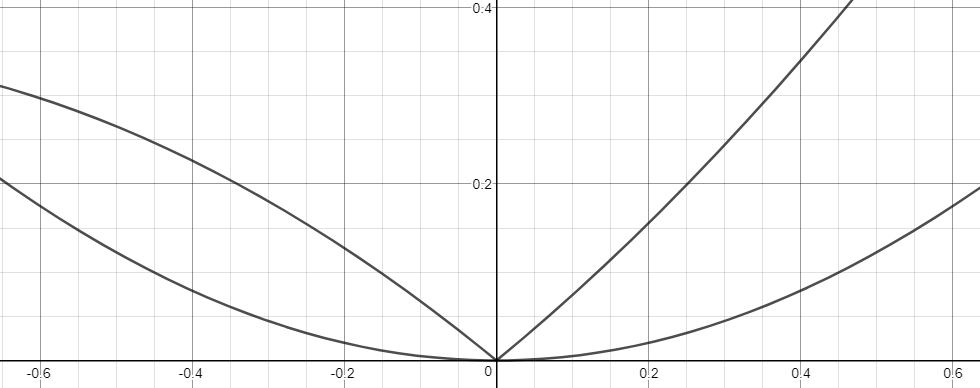
\includegraphics[width=3.26667in,height=1.29333in]{images/17_bell/contradiction.png}
  \end{center}
\end{figure}

The left-hand side ($1 + P(\pmb{b},\pmb{c})$) is the ``smooth'' curve, stationary at its minimum 
when $\pmb{b}=\pmb{c}$. The right-hand side is the V-shape that resembles the graph for 
$|\pmb{b}-\pmb{c}|$, and resembles it most when $|\pmb{b}-\pmb{c}|$ is small. The same basic shape 
is visible for different values of $\pmb{a}$ and $\pmb{b}$. For comparison, below is the graph of 
the case in which $\pmb{a}-\pmb{b}$ is equal to 22.5$^\circ$.

\begin{figure}[h]
  \begin{center}
    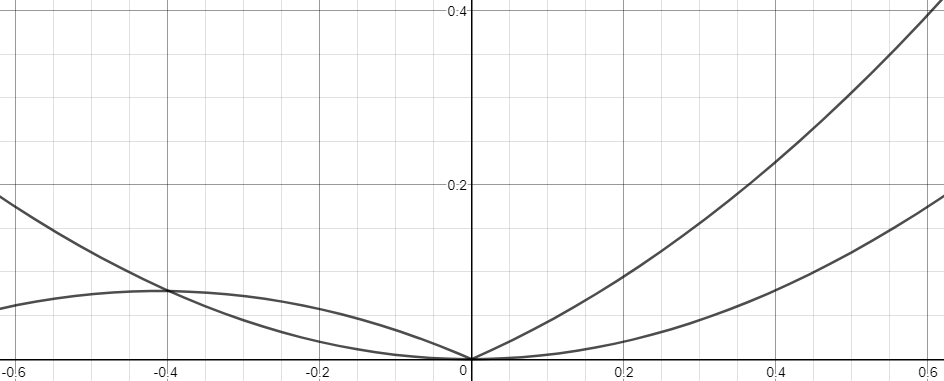
\includegraphics[width=3.14667in,height=1.27in]{images/17_bell/contradiction2.png}
  \end{center}
\end{figure}

Farther away from 0, the graph looks less like that of the absolute value function, but near 0,
it still has the characteristic pointiness due to the predominance of the linear term in $|\pmb{b}-\pmb{c}|$. 
Both graphs show the contradiction between the inequality (15), derived from both the local hidden
variables theory and the quantum-mechanical anti-correlation expressed in (13), and the quantum-mechanical
result in equation (3). Equation (15), therefore, does not count as what Bell means in section VI by ``a theory in which parameters are added to quantum mechanics to determine the results of individual measurements,
\emph{without changing the statistical predictions}.'' Equation (1), upon which (15) is based,
includes those added parameters and \emph{also} the "vital assumption" that the 
function $B$, specifying the result for the measurement of particle 2, ``does not depend on the setting $\pmb{a}$ of the magnet for particle 1, nor $A$ on $\pmb{b}$.'' The final result (15), however, contradicts those predictions expressed in (3).

\subsection*{The Same Thing, Otherwise}

We will demonstrate the quantum-mechanical violation of Bell's inequality experimentally, using
photons and not electrons as our particles, and polarization rather than spin as our measurement 
of interest. In Bell's and EPR's thought-experiments, the paired particles are in some way connected. 
In our experiment, we depend on the (obscure) mechanism of spontaneous parametric down-conversion to produce
pairs of photons that will exhibit the behavior a local hidden-variables theory implies is impossible. We have relied on this mechanism to produce pairs of photons before, but now we require them to be in a special state (akin to the ``singlet spin state'') that requires a different arrangement of our equipment.
%There's something unsatisfying about having to proceed without understanding the mechanism, 
%but our access to the phenomenon itself remains direct. Indeed, the results of our experiment will 
%themselves count as proof that the photons are, as is commonly said, "entangled," and therefore
%this is not something we need to be able to account for in order to ascertain.

In particular, we use a pair of down-conversion crystals oriented at 90$^{\circ}$ to each other, and pass laser light through them at a 45$^{\circ}$ angle to both, so that each can respond to the component of that light that is oriented along their relevant axes, producing a cone of pairs of photons. The two cones must be aligned spatially and in terms of their phase (by a ``compensating crystal'') by means of a process that the lab director can attest is lengthy and finicky.\footnote{The process is described in detail in parts IV, V, and VI of Dehlinger, D. and Mitchell, M.W., ``Entangled photons, nonlocality, and Bell inequalities in the undergraduate laboratory.'' \emph{Am. J. Phys.\ }\textbf{70} (9), 903--910 (2002).} The result of all this careful alignment is that, where the cones overlap, two paths are formed from the down-conversion crystals to the detectors. Along these paths are projected pairs of photons in a special state that has the same character as the particles in all our authors' thought experiments: a state which quantum mechanics describes as indeterminate but linked. Bell imagined testing two electrons produced according a process quantum mechanics says should give them indeterminate but opposed spin directions. Our apparatus produces photons that exhibit indeterminate but correlated polarization: when measured along a certain axis, they exhibit the same direction of polarization.


Because we are using photon polarization, our measurement scheme will have to be somewhat different.
In particular, Bell's function $P$, representing the average of the product of the results ($+1$ or $-1$)
of the measurements of electron spin, will have to be redefined. $A$ and $B$ still represent, so to
speak, a ``yes or no'' answer to the question put to each particle by the measuring device, but since
our equipment only detects ``yes'' answers, we will express (2) in terms of experimentally feasible 
tests. Let $A(\pmb{a},\lambda)$ be defined as equal to $+1$ when particle 1 is found to be polarized 
\emph{parallel} to $\pmb{a}$ (which state we'll denote as $V_a$), and equal to $-1$ when particle 1 
is found to be \emph{perpendicular} to $\pmb{a}$ (which state we'll denote as $H_a$, thinking of $\pmb{a}$
as ``vertical'' and its perpendicular as ``horizontal''), and let $B$ be defined similarly. We will call the 
probability that both particles are found to be polarized in the same direction as the specified measurement 
angles $P_{VV}$, the probability that the first is found to be polarized in the same direction as $\pmb{a}$ and the second perpendicular to $\pmb{b}$ 
$P_{VH}$, and so forth for the other two possibilities. The probabilities of each possible outcome, 
then, are
\begin{align*}
P_{VV}(\pmb{a},\pmb{b}) &= \int d\lambda\, \rho(\lambda) \frac{1+A(\pmb{a},\lambda)}{2}\frac{1+B(\pmb{b},\lambda)}{2}\\
P_{HH}(\pmb{a},\pmb{b}) &= \int d\lambda\, \rho(\lambda) \frac{1-A(\pmb{a},\lambda)}{2}\frac{1-B(\pmb{b},\lambda)}{2}\\
P_{VH}(\pmb{a},\pmb{b}) &= \int d\lambda\, \rho(\lambda) \frac{1+A(\pmb{a},\lambda)}{2}\frac{1-B(\pmb{b},\lambda)}{2}\\
P_{HV}(\pmb{a},\pmb{b}) &= \int d\lambda\, \rho(\lambda) \frac{1-A(\pmb{a},\lambda)}{2}\frac{1+B(\pmb{b},\lambda)}{2}.\\
\end{align*}
Bell calls his equation (2) the ``expectation value of the product,'' and in order to avoid possible confusion,
we will refer to this by the letter $E$, rather than $P$, which we've just used for the individual probabilities
of various outcomes. The overall expectation value of the product of the measurements $A$ and $B$, then, counting the correlations as positive and the anti-correlations as negative, is
\begin{equation*}\tag{R1}
E(\pmb{a},\pmb{b}) = \int d\lambda\, \rho(\lambda)\, A(\pmb{a},\lambda)B(\pmb{b},\lambda) = P_{VV}  + P_{HH} - P_{VH} - P_{HV}.
\end{equation*}
Effectively, what we have done is to factor $E(\pmb{a},\pmb{b})$ into four separate tests that we can perform directly, by setting up half-wave plates
in front of our detectors, each of which has a horizontal polarization filter in front of it. The
half-wave plates can be set so that light that has the polarization angle we want will have its
polarization rotated to the horizontal. This is helpful for ensuring the maximum sensitivity of our detectors by reducing the possibility of deflection caused by ordinary linear polarizing filters. In any case, the result is the same: photons polarized in the specified directions and arriving at the detectors within our specified time window will be detected and counted as simultaneous.

In one last deviation from Bell, we do not test his version of the inequality directly, but another
related one, derived on the same grounds, described here. Given four detection angles, $\pmb{a}$ and $\pmb{a'}$ 
for the first detector, and $\pmb{b}$ and $\pmb{b'}$ for the second, we define the quantity $s$, relevant
to the degree of correlation in direction of polarization in any given pair of photons:
\begin{align*}\tag{R2}
s \equiv& A(\pmb{a},\lambda)B(\pmb{b},\lambda) - A(\pmb{a},\lambda)B(\pmb{b'},\lambda) + A(\pmb{a'},\lambda)B(\pmb{b},\lambda)\\ 
     &+ A(\pmb{a'},\lambda)B(\pmb{b'},\lambda)\\
  =& A(\pmb{a},\lambda)[B(\pmb{b},\lambda)-B(\pmb{b'},\lambda)]\\
  &+ A(\pmb{a'},\lambda)[B(\pmb{b},\lambda)+B(\pmb{b'},\lambda)] 
\end{align*}
We will show that $s$ can equal only $-2$ or $+2$. Now, either $B(\pmb{b},\lambda) = B(\pmb{b'},\lambda)$ or $B(\pmb{b},\lambda) = -B(\pmb{b'},\lambda)$, given that each can only equal $+1$ or $-1$. Hence, of the two expressions in square brackets above,
one must be $0$ and the other $2$ or $-2$. Since $A$ can only be $+1$ or $-1$, $s$ as a whole can equal only
$+2$ or $-2$, which is what was to be demonstrated. Let us define $S$ as the average of $s$ over a set of pairs
of photons,
\begin{equation*}
S(\pmb{a},\pmb{a'},\pmb{b},\pmb{b'}) \equiv \; <s> \; = \int d\lambda\, \rho(\lambda)\, s(\lambda,\pmb{a},\pmb{a'},\pmb{b},\pmb{b'}),
\end{equation*}
and notice that this amounts to an expression in terms of expectation values $E$.
\begin{equation*}\tag{R3}
 S(\pmb{a},\pmb{a'},\pmb{b},\pmb{b'}) = E(\pmb{a},\pmb{b}) - E(\pmb{a},\pmb{b'}) + E(\pmb{a'},\pmb{b}) + E(\pmb{a'},\pmb{b'}). 
\end{equation*}
Given what we showed about the allowable values for $s$, and recalling that $\rho(\lambda)$ expresses the
probability of every possible value of $\lambda$, such that $\int d\lambda\, \rho(\lambda) = 1$, we can
be sure that 
\begin{equation*}\tag{R4}
|S| \leq 2.\footnotemark
\end{equation*}
\footnotetext{The derivation in these paragraphs is largely patterned after that found in Dehlinger and Mitchell, \emph{op. cit.} After the authors of the paper in which it first appeared (Clauser, Horne, Shimony, and Holt), (R4) is referred to as the CHSH inequality.}For us, this is what will play the role of Bell's equation (15). It embodies the assumption that measurements
on photon 1 depend on the setting of its detector ($\pmb{a}$) and some unknown parameters $\lambda$ that
together determine the result of the measurement, but not on the setting of detector 2, and vice versa. Unlike
in Bell's original derivation, there is nothing here that assumes anything about the relation of the
particles, as his equations (13) and (14) do. 

In these derivations, almost all of our manipulations (apart from some trigonometry and approximations of trigonometric functions) have been simple multiplications, additions, and subtractions. Arguably, the most arcane thing in the whole affair is integrating against the probability distribution $\rho(\lambda)$, but even this is simply a way of saying, ``whatever the various values of $\lambda$ that determine the outcomes of our measurements may be, let us duly account for all of them, weighting the more likely more and the less likely less.''


\section*{Practicum}

\subsection*{The Equipment}

\begin{itemize}
	
\item{a \emph{laser} that emits light at a wavelength of 405 nm,}

\item{\emph{mirrors} to direct the light in the right path,}

\item{a \emph{half-wave plate} (HWP), designed for 405 nm light, set to 45$^\circ$ so that the horizontally and vertically oriented down-conversion crystals will both receive light they can respond to,}

\item{a \emph{compensating crystal} (CC) which aligns the phase of the pairs emerging from the second down-conversion crystal with that of those emerging from the first,}

\item{a pair of beta-barium borate \emph{down-conversion crystals} (DC), rotated 90$^\circ$ relative to each other, to produce, by aid of the previous two components, photon \emph{pairs} in an \emph{indeterminate state} of linear polarization,}

\item{two \emph{half-wave plates} (HWP A/B), designed for 810 nm light, to rotate the polarization angles of the incoming photons,}

\item{two \emph{polarizing beam-splitters} (PBS) in front of the filters, set horizontally to allow suitably polarized light to enter the detectors,}

\item{two wavelength \emph{filters} in front of the detectors, to keep out stray photons, and}

\item{two sensitive light \emph{detectors} (A and B).}
	
\end{itemize}

\begin{figure}[h]
  \begin{center}
    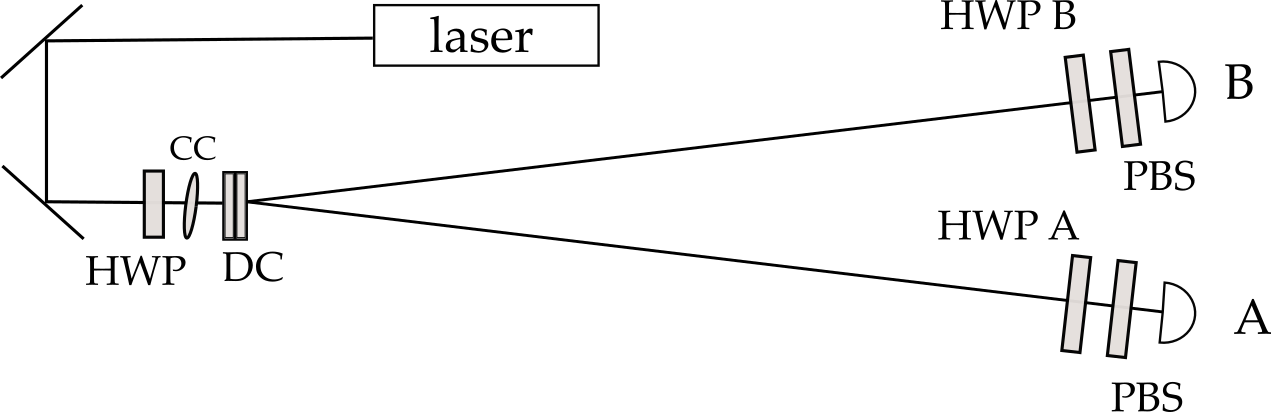
\includegraphics[width=4.23667in,height=1.37333in]{images/17_bell/bell-apparatus.png}
    \captionsetup{width=.75\textwidth}
    \caption*{\emph{Experimental setup for testing Bell's inequality.}}
  \end{center}
\end{figure}

We will measure $S$ using pairs of specially prepared photons, which (if all goes well) show a higher degree of
correlation of polarization direction than that allowed by (R4). To do that, we will have to measure
all the expectation values listed in (R3). We will measure each of those by measuring the probabilities
of the four outcomes in (R1), two correlations (with a positive sign) and two anti-correlations (with
a minus sign). All in all, then, we have to make 16 measurements. We shall measure these values using
an initial set of angles that is calculated to produce the greatest deviation from the inequality, namely:
\begin{equation*}
\pmb{a} = 0^\circ \;\;\; \pmb{a'} = \pi/4 = 45^\circ \;\;\;\pmb{b} = \pi/8 = 22.5^\circ 
\;\;\; \pmb{b'} = 3\pi/8 = 67.5^\circ.
\end{equation*}
For each expectation value $E$, we will count coincidences with four different settings of the detectors,
the original angles and their perpendiculars in all combinations. In what follows $\pmb{a}_\perp$ just
means $\pmb{a} + 90^\circ$ (what above we called $H_a$). To take an example at random, then, for 
$E(\pmb{a},\pmb{b'})$ we would take
measurements for equal times of the number of coincidences for each of the four settings, score the correlations as $+$ and the anti-correlations as $-$, i.e., tally them 
according to (R1), and finally divide that by the total number of coincidences for those four runs.
\begin{equation*}
E(\pmb{a},\pmb{b'}) = \frac{N(\pmb{a},\pmb{b'}) + N(\pmb{a}_\perp,\pmb{b'}_\perp) - N(\pmb{a},\pmb{b'}_\perp) - N(\pmb{a}_\perp,\pmb{b'})}{N(\pmb{a},\pmb{b'}) + N(\pmb{a}_\perp,\pmb{b'}_\perp) + N(\pmb{a},\pmb{b'}_\perp) + N(\pmb{a}_\perp,\pmb{b'})}
\end{equation*}
For convenience, here is a sample table of all the settings and measurements, with space to record results.
The example calculation above would be for rows 5 through 8. You will notice that the half-wave plates 
(listed as ``hwp'') have to be set to half the desired angle. Perform 2 or 3 runs for each trial. Whichever you choose, perform the same number of equally timed runs for all 16 trials.

\begin{center}
	\begin{tabular}{| r | l  l | l | l || l | l | l | l |}
	\toprule
	\# &  &  & A & hwp & B & hwp& Counts \;\; (30 seconds)& $\pm$\\ \toprule
	1&$\pmb{a}$&$\pmb{b}$&$0$&$0$&$22.5$&$11.25$& &$+$\\ \hline
	2&$\pmb{a}_\perp$&$\pmb{b}$&$90$&$45$&$22.5$&$11.25$& &$-$\\ \hline
	3&$\pmb{a}$&$\pmb{b}_\perp$&$0$&$0$&$112.5$&$56.25$& &$-$\\ \hline
	4&$\pmb{a}_\perp$&$\pmb{b}_\perp$&$90$&$45$&$112.5$&$56.25$& &$+$\\ \toprule
	5&$\pmb{a}$&$\pmb{b'}$&$0$&$0$&$67.5$&$33.75$& &$+$\\ \hline
	6&$\pmb{a}_\perp$&$\pmb{b'}$&$90$&$45$&$67.5$&$33.75$& &$-$\\ \hline
	7&$\pmb{a}$&$\pmb{b'}_\perp$&$0$&$0$&$157.5$&$78.75$& &$-$\\ \hline
	8&$\pmb{a}_\perp$&$\pmb{b'}_\perp$&$90$&$45$&$157.5$&$78.75$& &$+$\\ \toprule
	9&$\pmb{a'}$&$\pmb{b'}$&$45$&$22.5$&$67.5$&$33.75$& &$+$\\ \hline
	10&$\pmb{a'}_\perp$&$\pmb{b'}$&$135$&$67.5$&$67.5$&$33.75$& &$-$\\ \hline
	11&$\pmb{a'}$&$\pmb{b'}_\perp$&$45$&$22.5$&$157.5$&$78.75$& &$-$\\ \hline
	12&$\pmb{a'}_\perp$&$\pmb{b'}_\perp$&$135$&$67.5$&$157.5$&$78.75$& &$+$\\ \toprule
	13&$\pmb{a'}$&$\pmb{b}$&$45$&$22.5$&$22.5$&$11.25$& &$+$\\ \hline
	14&$\pmb{a'}_\perp$&$\pmb{b}$&$135$&$67.5$&$22.5$&$11.25$& &$-$\\ \hline
	15&$\pmb{a'}$&$\pmb{b}_\perp$&$45$&$22.5$&$112.5$&$56.25$& &$-$\\ \hline
	16&$\pmb{a'}_\perp$&$\pmb{b}_\perp$&$135$&$67.5$&$112.5$&$56.25$& &$+$\\ \toprule


\end{tabular}
\end{center}

\section*{Conclusion}

Since the first experimental verification that at least some specially prepared particles violate Bell's inequality, there have been many developments and refinements. In the most significant recent tests, many of the ``loopholes'' that critics have pointed out over the years have been closed.\footnote{E.g., M. Giustina \emph{et al.}, 
``Significant loophole-free test of Bell's theorem with entangled photons,'' \emph{Phys. Rev. Lett.}\  
\textbf{115} (2015), and B. Hensen \emph{et al.}, ``Loophole-free
Bell inequality violation using electron spins separated by 1.3 km,'' \emph{Nature} \textbf{526}, 682--686 (29 Oct. 2015).}
Reflection on the significance of this particular state of particles, which is commonly referred to as ``entanglement,'' has become a standard feature of discussions of the results of scientific inquiry into the behavior of electrons and photons and the quantum-mechanical theories that purport to explain it.
